% !TEX program=lualatex
\RequirePackage{luatex85}
\documentclass{article}
\usepackage{amsmath}
\usepackage[letterpaper,margin=1in]{geometry}
\usepackage{url}
\usepackage{graphicx}
\usepackage[utf8]{inputenc}
\usepackage[T1]{fontenc}
\usepackage[style=nature, citestyle=authoryear]{biblatex}
\usepackage{tikz}
\usepackage{wrapfig}
\usepackage{lineno}
\usepackage{outline}
\usepackage{tabularx}
\bibliography{citations.bib}
\graphicspath{./figures/}

\begin{document}
\linenumbers

\section{Introduction}

\begin{outline}
	%paragraph level
	\item DNA sequencing and applications
	\begin{outline}
		\item Next generation sequencing has a plethora of applications in biology. %TODO: give some examples
		\item While the technology is widely applied, current technology is inherently erroneous and errors are common in sequencing data, with base substitution error rate estimates ranging between $.1$ and $1\%$, depending on the sequencing technology used. %TODO: cite
		\item To help mitigate this, DNA molecules are usually copied and sequenced multiple times to ensure the sequence is correct, since multiple independent measurements are unlikely to all contain the same error at the same position. While this works well in general, it can be costly and additional sample manipulation can damage samples and insert mutations, further increasing the amount of technical error in the data. %TODO: cite
	\end{outline}
\end{outline}

\subsection{Quality Scores}

\begin{outline}
	\item What are quality scores and why are they important? \parencite{ewing_base-calling_1998} \parencite{ewing_base-calling_1998-1}
	\begin{outline}
		\item In addition to increased sequencing depth, quality scores are an important part of sequencing data that helps identify erroneous sequences. Sequencing data is usually presented along with quality scores in the Phred scale \parencite{ewing_base-calling_1998, ewing_base-calling_1998-1}.
		\item These quality scores measure the confidence the instrument has in its determination that any particular base in the sequence is correct.
		\item Specifically, the quality score is equal to $-10\log_{10}P(e)$ \parencite{ewing_base-calling_1998} \parencite{ewing_base-calling_1998-1}, where $P(e)$ is the probability the base is an error.
		\item For example, a base with a quality score of 40 has a .0001 probability of being incorrect while a base with a quality score of 10 has probability .1 of being incorrect. Generally, bases with scores lower than 10 are considered bad quality and bases with scores 30 and above are considered to be good quality. However, the score allows finer resolution than "good" and "bad", and is therefore more nuanced.
		%new paragraph - importance
		\item The usefulness of quantitative scores over categorical can be illustrated by considering how variant calling algorithms utilize quality scores.
		\item Variant calling is a task to identify genetic variation in a sample from sequencing data.
		\item Variant calling models use quality scores to differentially weight the observed data. Generally, these models attempt to find the sample genotype most consistent with the observed data and recognize that low quality bases provide less reliable evidence for one genotype over another. The BCFTools multiallelic caller \parencite{li_sequence_2009}, GATK's HaplotypeCaller \parencite{poplin_scaling_2018}, and FreeBayes \parencite{garrison_haplotype-based_2012}---three of the most popular variant callers---all take quality score into consideration when calling variants.
		\item Since the quality score is an exactly defined probability, it is straightforward to integrate these scores into a model.
		%new paragraph - binning
		\item If so desired, quantitative scores can be collapsed into coarser categories, such as "good" and "bad". This is sometimes done as a heuristic; \textit{ie.} scores less than 10 are untrustworthy and filtered out of a dataset and other scores are trusted and retained.
		\item The practice of binning quality scores together with neighboring scores is commonly performed to reduce file size. %TODO: cite. there is an Illumina paper about this.
		\item However, it's important to note that this process cannot be simply reversed as information is lost when the scores are binned.
		% \item Quality score resolution can be increased through a process called Base Quality Score Recalibration.
		% \item The data generated is produced in the FASTQ format \parencite{cock_sanger_2010}, which is a multi-line format that combines the sequence output by the instrument with a score for each base indicating the quality of that base.
		% \item Quality score binning
		% \item Variant calling has applications in many fields including medicine, evolution, and conservation.
	\end{outline}
\end{outline}

\subsection{Base Quality Score Recalibration}

\begin{outline}
	\item What is Base Quality Score Recalibration?
	\begin{outline}
		\item While base quality scores are important for identifying reliable data, base quality scores are often incorrect.
		\item Base quality scores are exactly defined as a probability. They can be interpreted as a prediction giving the probability the reported base is an error. In general, probabilities are called \textit{calibrated} if the reported probability accurately predicts the frequency of an event.
		\item Base quality scores in Illumina sequencing reads are not well-calibrated \parencite{callahan_dada2:_2016}. %(TODO: more cites)
		\item A few alternative base calling models have been developed for Illumina machines that improve base call accuracy and quality score calibration; however, these are difficult to use because they require the raw output from the sequencing machine, which is unavailable to most users of sequencing as they are usually disposed of after a sequencing run due to the large cost associated with storing that data. %TODO: cite
		%New para
		\item Since base quality scores are used to some degree by most variant calling methods, it is probable that poorly calibrated reads reduce the quality of resulting variant calls.
		\item Similarly, the reduced amount of information in binned quality scores may also impact the quality of variant calls made using the data.
		\item Poor calibration combined with poor resolution resulting from quality score binning may have an important impact on algorithms that rely on these scores to function, but the exact affect of these phenomena are unknown.
		% new paragraph - actual BQSR
		\item Though increased sequencing depth can help mitigate the impact of random sequencing errors, sequencing is affected by non-random biases. %todo: cite
		\item For these types of errors, increasing sequencing depth counterintuitively \textit{increases} the effect of these errors, as they by definition occur preferentially at the same location. Thus, increased sequencing depth at that location adds more errors than are expected by chance, making those erroneous reads seem trustworthy. 
		\item These biases can be due to the nature of the DNA sequence itself, with errors induced during library preparation or the sequencing reaction likely due to secondary structure \parencite{meacham_identification_2011, nakamura_sequence-specific_2011}.
		\item At the same time, the sequencing reaction is also non-randomly biased. Bases at the end of a read are much more likely to be erroneous than bases at the beginning of the read, and the identity of the base and adjacent bases also affect the error rate. %todo: cite
		\item Thus while random errors are troublesome, their impacts can be somewhat mitigated by more sequencing. Systematic errors cannot addressed in the same way, but they can be modeled.
		%discuss non-random genomic locus vs. sequencing characteristics etc.    %non-random errors
	\end{outline}
	\item GATK BQSR occurs in 3 phases.
	\begin{outline}
		% Phase 1 - Count errors and covariates
		\item Base quality score recalibration (BQSR) is the process of modeling errors in sequencing data and using the created model to update quality scores such that they reflect an accurate probability of error of any base.
		\item GATK BQSR  is the most popular method for BQSR and is recommended before variant calling by the GATK best practices. %todo cite
		\item The model integrates many covariates of error such that the output quality score reflects an accurate, independent measure of the probability of error.
		\item The algorithm takes reads aligned to a reference and a database of potentially variable sites in the genome as input.
		\item The algorithm proceeds in 3 phases.
		\item In the first phase, the algorithm compares each read to the aligned reference. Potentially variable sites are ignored and mismatches from the reference sequence and non-mismatches are counted. The numbers of matching and mismatching bases are categorized according to the model covariates, which are: read group, assigned quality score, sequencing cycle, and the base identity along with the identity of the previous base (the base context).
		% Phase 2 - Train a hierarchical model.
		\item In the second phase, a bayesian hierarchical model is trained with the count data. Using a normal distribution of the mean probability of error as a prior, the \textit{maximum a posteriori} (MAP) quality score of the read group is calculated assuming the errors are binomially distributed. That is,
		\begin{align}
		\hat{Q}_{rg} &= \operatorname{argmax}_{Q_{rg}} P(Q_{rg}|Errors_{rg}) \\
		&= \operatorname{argmax}_{Q_{rg}} P(\mathcal{B}(Errors_{rg} | Observations_{rg}, Q_{rg}) * P(\mathcal{N}(Q_{rg} | \bar{Q}))
		\end{align}
		\item This score is then used as the prior for calculating the \textit{maximum a posteriori} quality score for each assigned quality score in that read group, $\hat{Q}_{assigned\:quality\:score}$, using a simular formula.
		\item In turn, this score is used as the prior for calculating the \textit{maximum a posteriori} scores for the sequencing cycle and context covariates of bases with that score. The difference between the MAP estimate and the prior is used to calculate the final score, which is the sum of the MAP estimate of the assigned quality score and these two differences. That is,
		\begin{align}
		\Delta Q_{cycle} &= \hat{Q}_{cycle} - \hat{Q}_{assigned\:quality\:score} \\
		\Delta Q_{context} &= \hat{Q}_{context} - \hat{Q}_{assigned\:quality\:score} \\
		Q_{recalibrated} &= \hat{Q}_{assigned\:quality\:score} + \Delta Q_{cycle} + \Delta Q_{context}
		\end{align}
		\item In the third phase, the quality score of each read is adjusted based on the four covariates for each base in the read according to values calculated in the previous phase.
	\end{outline}
	\item How much does BQSR help?
	\begin{outline}
		\item BQSR improves quality score calibration in many cases, especially when there is moderate sequencing depth and the database of variable sites is nearly complete. %todo : cite
		\item While BQSR is recommended in GATK's Best Practices, its affect on the resulting variant calls is not well-characterized, and there is ongoing debate about whether to continue recommending BQSR. \parencite{van_der_auwera_geraldine_2020} %todo: more cites
		\item However, \cite{ni_improvement_2016} find that improved quality score calibration aids detection of minor alleles in high coverage datasets by increasing sensitivity and reducing the number of false positive calls.
		\item Thus, the need to perform BQSR and the performance of GATK's BQSR algorithm may vary from study to study.
		\item One objective of this work is to help elucidate when GATK BQSR performs well and when it fails, and provide a method that works in situations that GATK BQSR struggles with.
		\item As an example, the GATK developers recommend BQSR for use in cancer variant discovery \parencite{cibulskis_sensitive_2013}, but the tumor genome is likely much different from the human genome, and the database of variable sites will likely miss many truly variable sites due to the large mutation rate present in cancer genomes. Additionally, mismatches in reads misaligned due to chromosomal rearrangements may be mistakenly counted as evidence of sequencing error. The number of these errors required to significantly impact the performance of the algorithm is not clear.
	\end{outline}
\end{outline}

\subsection{Alternative Approaches for BQSR}

\begin{outline}
	\item What is the problem with current methods for BQSR?
	\begin{outline}
		\item As illustrated above, the most problematic aspect of GATK BQSR occurs in the first phase of the algorithm: counting erroneous and non-erroneous bases. This is especially true when considering non-model organisms, where alignment errors may be common. Furthermore, in non-model organisms a database of variable sites is likely unavailable or largely incomplete. However, there are methods that attempt to overcome this deficiency. While there exist alternative approaches that implement different error models, such as Lacer \parencite{chung_lacer:_2017}, the biggest problem for analyzing data without reliable reference information is the method of counting erroneous and non-erroneous bases.


		% \item In a variant calling context, BQSR is probably most helpful in regions with low coverage, as the limited amount of data makes it difficult to differentiate between errors, heterozygous sites, and mutations.
		 % or inconsistent coverage, as one may expect when sequencing a non-model organism; however, by definition that means no quality reference nor database of variable sites are available. Since these are required to perform GATK's BQSR, that means BQSR cannot be confidently completed.
		% \item Find some estimates of differences between reference and samples sequenced; perhaps look at mouse
		% \item This will be highly species-dependent and situation specific
	\end{outline}
	\item Alternative Approaches
		\begin{outline}
		\item Many alternative algorithms have been developed to avoid providing a database of variable sites. However, these approaches all still require a reference and alignment, and many require extra reagents and sequencing that increases the cost of analysis and cannot be used to reanalyze existing sequencing data that hasn't been specially prepared.
		% \item Lacer \parencite{chung_lacer:_2017} bins aligned bases based on depth and whether the base matches the reference, then uses singular value decomposition to infer the shift in quality score for each base.
		\item ReQON \parencite{cabanski_reqon:_2012}, like GATK, considers bases that do not match the reference as errors but limits the number of acceptable errors at a position to minimize the effect of unknown variants. It then uses a logistic regression to recalibrate the quality scores.
		\item SOAP2 \parencite{li_soap2:_2009} contains a model for consensus sequence construction that performs BQSR during construction. %It doesn't seem possible to get these recalibrated scores out??
		\item The methods of \cite{zook_synthetic_2012} and \cite{ni_improvement_2016} use synthetic spike-ins of known composition and GATK's model \cite{zook_synthetic_2012} or piecewise regression \parencite{ni_improvement_2016} to recalibrate quality scores. Since the sequence of the spike-in is known before hand, errors are easy to identify as there should be no biological variation in the spiked-in sample.
		% \item While these approaches are useful alternatives to GATK, the comparisons presented here will only compare against GATK BQSR as none of the alternative approaches function without a reference and GATK BQSR is the most popular method.
		\item Crucially, these methods require a reference and possibly other information to recalibrate reads that may not be available.

		\end{outline}
	\item Here we present \texttt{kbbq}, a software package to recalibrate quality scores of whole genome sequencing data without a reference or database of variable sites. The only required input is the set of reads to be recalibrated. Rather than excluding variation and comparing to the reference like GATK does, \texttt{kbbq} uses k-mer subsampling to find likely errors. Once the number of errors and nonerrors are counted and categorized according to their covariates, it uses the same model GATK uses to recalibrate the reads. I show how simulated false negatives and false positives affect GATK's ability to recalibrate reads and compare GATK calibration to \texttt{kbbq}.
\end{outline}
\section{Materials and Methods}
\begin{outline}
	% \item Error correction algorithms
	\item \texttt{kbbq} performs BQSR by adjusting how errors in the dataset are discovered.
	\begin{outline}
		\item Instead of looking at the reference, \texttt{kbbq} implements the error-correction algorithm described in \cite{song_lighter_2014} and uses the errors detected by that procedure to train and apply the standard GATK model. Note that the sequenced bases are not actually changed; the detected errors are used only to train the model. If there is evidence according to the model that the base is erroneous, its base quality will be decreased according to the strength of that evidence.
		\item Briefly, the algorithm subsamples k-mers from the dataset. Since erroneous k-mers are expected to be unique, erroneous k-mers are less likely to be sampled than error-free k-mers. A binomial test is then conducted for every nucleotide in the dataset; if a sufficient number of k-mers contain the nucleotide, the base is likely not erroneous and called trusted. If \textit{k} of these trusted bases appear next to each other, that k-mer is stored as a trusted k-mer. Once the trusted k-mers have all been stored, each read is iterated through once again and any bases on the edge of an island of trusted k-mers are changed such that the change produces the maximal number of trusted k-mers in the read. These changes are marked as errors and used to train the model.
		\item The model training and recalibration procedure are the same as those described above for GATK's BQSR method.
	\end{outline}
\end{outline}
\subsection{Program Input and Parameters}
\begin{outline}
	\item \texttt{kbbq} requires as input a set of reads in FASTQ \parencite{cock_sanger_2010} or BAM \parencite{li_sequence_2009} format. If the input data is FASTQ formatted and consists of multiple read groups, the read group each read belongs to should be annotated in the name of each read. Alternatively, if the user has an original data file and a data file that has already been corrected using an error correction program, the user may supply the corrected file with the \texttt{-\phantom{}-fixed} option to obtain errors from that correction rather than performing the error correction algorithm included in \texttt{kbbq}. The program's only required parameter is the approximate length of the sequenced region in base-pairs, and this information can be taken from the BAM header if it is present. It may be set with the \texttt{-\phantom{}-genomelen} option. If BAM input is provided, the \texttt{-\phantom{}-set-oq} and \texttt{-\phantom{}-use-oq} flags can be used to set the OQ flag on the read before recalibrating or to use the quality scores encoded in the OQ flag rather than the quality scores in the primary quality score field.

	\item Optionally, the approximate sequencing coverage may also be provided with the \texttt{-\phantom{}-coverage} option. If it is not, it will be estimated by finding the length of the sequenced data divided by the provided genome length; $\operatorname{Coverage} = \frac{\operatorname{Sequence\:Length}}{\operatorname{Genome\:Length}}$.
	\item An $\alpha$ parameter may also be provided with the \texttt{-\phantom{}-alpha} option; this is the same $\alpha$ parameter that Lighter uses, and is the fraction of reads sampled from the input data \parencite{song_lighter_2014}. If not provided, the recommended value of $\alpha = \frac{7}{\operatorname{Coverage}}$ is used.
	\item A $\texttt{-k}$ parameter may also be provided, which changes the k-mer size used for the error detection algorithm. The maximum value of 32 is recommended and is the default value.
	\item A summary of flags and options the program supports is listed in table \ref{table:params}.
	%new para
	\item The genome length parameter, in addition to being used to estimate sequencing coverage, is also used to estimate the number of k-mers that will be sampled. This is used to parameterize the bloom filter that stores the sampled and trusted k-mers. This parameterization is different than that used in Lighter; there, the number of sampled k-mers is estimated to be $1.5 \times \operatorname{Genome\:length}$. However, the expected number of sampled k-mers $K_{\operatorname{sampled}}$ is bounded by the expected value of the binomial distribution parameterized by $\operatorname{Genome\:length} \times \operatorname{Coverage}$ and $\alpha$. Assuming \textit{every} k-mer is unique, the number of possible k-mers in the dataset $K_{\operatorname{total}}$ is less than $\operatorname{Coverage} \times \operatorname{Genome\:length}$. Since the number of k-mers in each read is $\operatorname{Read\:length} - k + 1$ and assuming equal read lengths, the total number of k-mers is:
	\begin{align}
	K_{\operatorname{total}} &= \sum_{\operatorname{Reads}}{\operatorname{Read\:length} - k + 1} \\
	&= (\operatorname{Read\:length} - k + 1) \times \operatorname{Number\:of\:reads} \\
	&< \operatorname{Read\:length} \times \operatorname{Number\:of\:reads} \\
	&< \operatorname{Read\:length} \times \frac{\operatorname{Coverage} \times \operatorname{Genome\:length}}{\operatorname{Read\:length}} \\
	&< \operatorname{Coverage} \times \operatorname{Genome\:length}
	\end{align}

	\item So the expected number of sampled k-mers is

	\begin{align}
	E[K_{\operatorname{sampled}}] &= E[\mathcal{B}(x; \alpha, K_{\operatorname{total}})] \\
	&= \alpha \times K_{\operatorname{total}} \\
	&< \alpha \times \operatorname{Coverage} \times \operatorname{Genome\:length}
	\end{align}

	\item Notably, if $\alpha$ is the recommended value of $\frac{7}{\operatorname{Coverage}}$, the expected number of sampled k-mers is less than $7 \times \operatorname{Genome\:length}$, a bound over 4 times larger than the estimate used by Lighter. For the data analyzed here, this provides a much better estimate of the true number of sampled k-mers. Ultimately, the larger estimate of elements inserted into the bloom filter causes an increase in size of the bloom filter but a smaller false positive rate.

\end{outline}

	\begin{table}
	\begin{tabularx}{\textwidth}{| l | l | >{\hsize=.7\hsize\linewidth=\hsize}X | >{\hsize=1.3\hsize\linewidth=\hsize}X | }
	\hline
	\textbf{Parameter} & \textbf{Short Option} & \textbf{Default Value} & \textbf{Summary} \\
	\hline
	\texttt{-\phantom{}-ksize} & \texttt{-k} & 32 & Size of k-mer to use for correction\\
	\texttt{-\phantom{}-use-oq} & \texttt{-u} & Off & Use BAM OQ values as quality scores\\
	\texttt{-\phantom{}-set-oq} & \texttt{-s} & Off & Set BAM OQ values before recalibration\\
	\texttt{-\phantom{}-genomelen} & \texttt{-g} & Estimated for BAM, \newline required for FASTQ & The approximate size of the sequenced region in base-pairs.\\
	\texttt{-\phantom{}-coverage} & \texttt{-c} & Estimated from data & Approximate sequencing coverage\\
	\texttt{-\phantom{}-fixed} & \texttt{-f} & Off & Treat changes to reads in the given file as errors and recalibrate. \\
	\texttt{-\phantom{}-alpha} & \texttt{-a} & 7 / coverage & Rate to sample k-mers\\
	\hline
	\end{tabularx}
	\caption{\texttt{kbbq} parameters, short options for each long parameter name, the default value of the parameter and a summary of how each parameter changes the behavior of the program.}
	\label{table:params}
	\end{table}

\subsection{Testing and Validation}
\begin{outline}
	\item Describe test dataset used for benchmarking.
	\begin{outline}
		\item To test the performance of \texttt{kbbq}, I reanalyzed the synthetic diploid CHM1-CHM13 dataset from \cite{li_synthetic-diploid_2018}. Like other benchmarking datasets, this dataset includes a BED file describing confident regions in which the genotype of any site that differs from homozygous reference within those regions are included in a VCF file. For the purposes of this work, I assume these confident regions and associated VCF entries are correct and represent the true genotype of the sequenced sample.
		\item This dataset was specifically designed to study the impact of deep sequencing on variant calling and has a coverage of approximately 45x. Thus, the affect of sequence specific errors and other non-random biases in sequencing should be pronounced in this data.
		\item The dataset was constructed by adding equal concentrations of DNA of CHM1 and CHM13 human complete hydatidiform mole cell lines and sequencing the mixture. These moles are formed when a sperm combines with an egg containing no nucleus; the sperm then undergoes mitosis to generate a completely homozygous cell mass. They are effectively haploid, and it is significantly easier to genotype a haploid cell than a diploid one. Thus, the mixture simulates a diploid human cell but the genotype of each "haplotype" is known. This means there should be very few, if any, errors in the declared genotypes included with the data. This is what \cite{li_synthetic-diploid_2018} find when validating their data as well.
		%new paragraph
		\item To measure the performance of \texttt{kbbq} and compare to GATK's BaseRecalibrator and ApplyBQSR tools, I subset the full dataset to only reads aligned on Chromosome 1 and overlapping the BED of confident regions using the samtools view command \parencite{li_sequence_2009}. I then used the samtools fixmate and view commands to remove any singleton reads. I then ran \texttt{kbbq} on the dataset with the options \texttt{-\phantom{}-use-oq -g 214206308 -a .15}. I also ran GATK's BaseRecalibrator with the provided variant data as the known sites file and the \texttt{-\phantom{}-use-original-qualities} flag set. I then used the ApplyBQSR tool with the \texttt{-\phantom{}-use-original-qualities} flag to recalibrate the input file. I then compared the two recalibrated files by running the BaseRecalibrator tool again with the same options on both output datasets and using GATK's AnalyzeCovariates tool.
		%new paragraph
		\item In order to determine how misspecification of the database of variable sites affects the calibration of GATK's BQSR procedure, I simulated various levels of false negative and false positive variants. In this case, false negative variants in the database of variable sites causes a site that should be ignored to not be ignored, greatly increasing the number of bases that GATK classifies as sequencing errors. On the other hand, false positive variants remove a site from GATK classification, so the affect is likely to be small except for large false positive rates. To create each false negative dataset, an appropriate number of sites from the VCF were randomly sampled with BCFTools and the shuf program. To create each false positive dataset, all sites from the VCF were extracted in BED format with the BCFTools query command, then subtracted from the BED of confident regions with bedtools subtract \parencite{quinlan_bedtools_2010}. The appropriate number of sites were then sampled with the shuf program and appended to the sites from the VCF to generate the BED file of all sites to exclude. These files were then provided as input to GATK the GATK BaseRecalibrator and calibration was evaluated with GATK's AnalyzeCovariates.
	\end{outline}
\end{outline}
\section{Results}
\begin{outline}
	\item Simulate false positives in database of variable sites and summarize degree of miscalibration (brier score and RMSE)
	\begin{outline}
		\item \includegraphics[width = 5in]{./figures/fpr.pdf}
		\item Base quality score calibration for a range of false positives in the database of variable sites. The false negative rate is zero. Increasing the false positive rate does not significantly impact the quality of the calibration.
	\end{outline}
	\item Simulate false negatives in database of variable sites and summarize degree of miscalibration (brier score and RMSE)
	% \begin{figure}[h]
	\begin{outline}
		\item 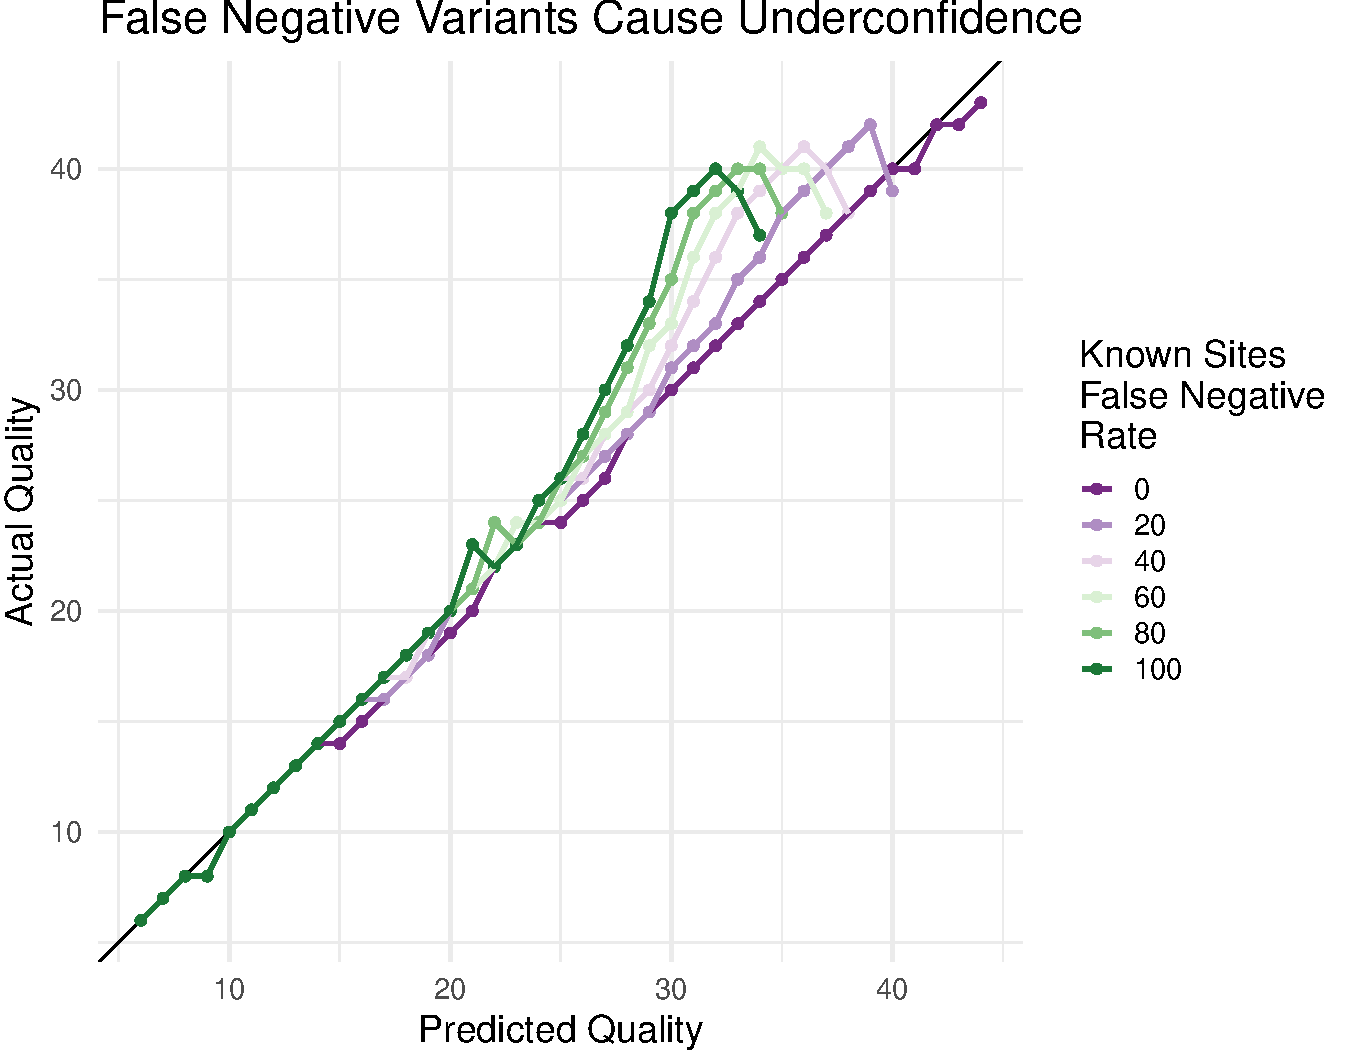
\includegraphics[width=5in]{./figures/fnr.pdf}
		\item Base quality score calibration for a range of false negatives in the database of variable sites. The false positive rate is zero. Increasing the false negative rate decreases the quality of the calibration.
		% \caption{Base quality score calibration for a range of false negatives in the database of variable sites. The false positive rate is zero. Increasing the false negative rate decreases the quality of the calibration.}
	% \end{figure}
	\end{outline}	
	\item Simulate both false positives and negatives and summarize degree of miscalibration.
	% \item Simulate downstream effect of FP and FN on variant quality; perhaps can do this with F-score - this should be done for CH3
	% \item Perhaps look at depth vs. variant quality to see if BQSR helps more in low-coverage scenarios - this should be done for CH3
	\item Summarize FP / FN / and FP+FN results in a table
	\item Application
	\begin{outline}
		\item Describe Eucalyptus data
		\item Describe structure in data that enables estimating the false positive and false negative rate
		\item Recalibrate reads with \texttt{kbbq} instead of GATK BQSR and see how variant FPR and FNR change.
	\end{outline}
\end{outline}
\section{Discussion}
\begin{outline}
	\item GATK BQSR can cause miscalibration worse than using raw data in some situations
	\item GATK BQSR is vulnerable to false negatives in the known sites input.
	\begin{outline}
		\item False negatives are likely to be numerous \parencite{bobo_false_2016} in nearly any case except with data generated from human samples.
		\item GATK best practices recommends using only the most confident variants called from uncalibrated reads to use for recalibration in the case that a database of sites is not available.
	\end{outline}
	\item \texttt{kbbq} is resilient to misspecified references and missing databases of variable sites, since it doesn't use those as input.
	\item Compare simulated scenarios to non-model and cancer scenarios?
	\begin{outline}
		\item In situations where the sample may not closely match the reference, use \texttt{kbbq} or don't recalibrate.
	\end{outline}
	\item Future work: see how big the difference is in variant calls using binned quality scores, miscalibrated reads, and well calibrated reads.
\end{outline}

\printbibliography


\end{document}
